%!TEX root = ../main.tex

\section{Results and discussion}

This section provides results and related discussions for the effects of different fluidization gases on the operation and conversion of a bubbling fluidized bed reactor.

\subsection{Comparison of gas properties}

Molecular weight, viscosity, density, thermal conductivity, heat capacity, and Prandtl number of the individual gases investigated in this paper are shown in Figure \ref{fig:gas-properties}. The gas properties were calculated at a pressure of 101,325 Pa and a temperature of 773.15 K (500$^\circ$C). The lightest gas in terms of molecular weight and density is hydrogen while the heaviest gas is carbon dioxide. The highest viscosity is noted for the nitrogen gas while hydrogen has the lowest viscosity. The largest thermal conductivity is for hydrogen at approximately 0.36 W/(m\,K) while the other gases remain below 0.12 W/(m\,K). The highest heat capacity is obtained for methane at 62 J/(mol\,K) while the lowest is for hydrogen at 29 J/(mol\,K). The Prandtl number is similar for all the gases except for water vapor.

\begin{figure}[H]
    \centering
    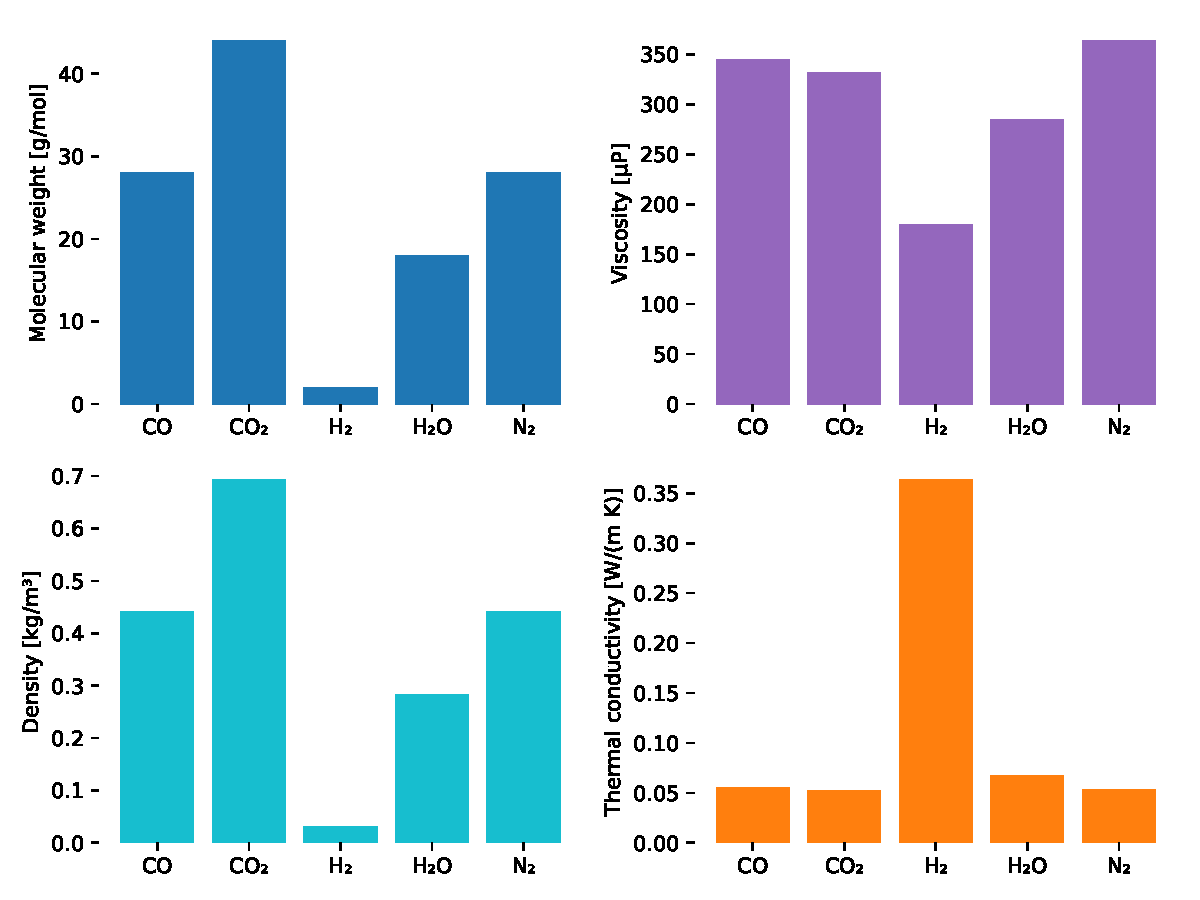
\includegraphics[width=\textwidth]{gas-properties.pdf}
    \caption{Comparison of molecular weight (MW), viscosity ($\mu$), density ($\rho$), thermal conductivity (k), heat capacity (Cp), and Prandtl number (Pr) for each gas at 101,325 Pa and 773.15 K (500$^\circ$C).}
    \label{fig:gas-properties}
\end{figure}

Properties for molecular weight, viscosity, and density for the gas mixtures investigated in this paper are shown in Figure \ref{fig:mix-properties}. Similar to the individual gas properties, the mixture properties were calculated at 101,325 Pa and 773.15 K (500$^\circ$C). The fraction of each gas in the mixture is given by the values shown at the top of each column in the figure. For example, the hydrogen and nitrogen mixture is comprised of 80\% hydrogen and 20\% nitrogen which is labeled as $0.8 + 0.2$. As expected, the carbon dioxide mixture is the heaviest in terms of molecular weight and density.

\begin{figure}[H]
    \centering
    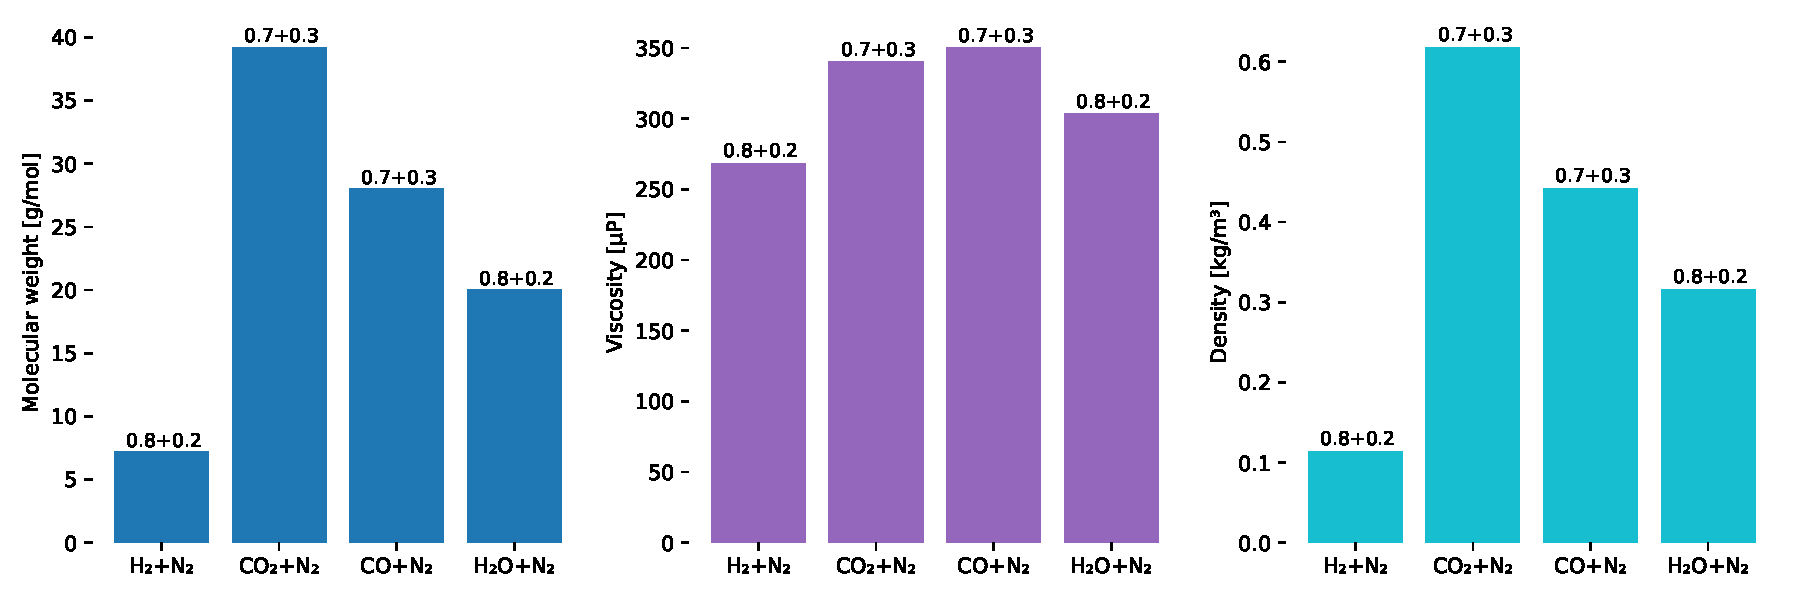
\includegraphics[width=\textwidth]{mix-properties.pdf}
    \caption{Comparison of gas mixture properties for molecular weight, viscosity, and density at 101,325 Pa and 773.15 K. Fraction of each gas component is shown at the top of each column.}
    \label{fig:mix-properties}
\end{figure}

\subsection{Fluidization effects}

Minimum fluidization velocity (Umf) of the bed material for the different fluidization gases is presented in Figure \ref{fig:gas-umf}. The hydrogen gas requires about twice the gas velocity to fluidize the sand bed compared to the nitrogen gas.

\begin{figure}[H]
    \centering
    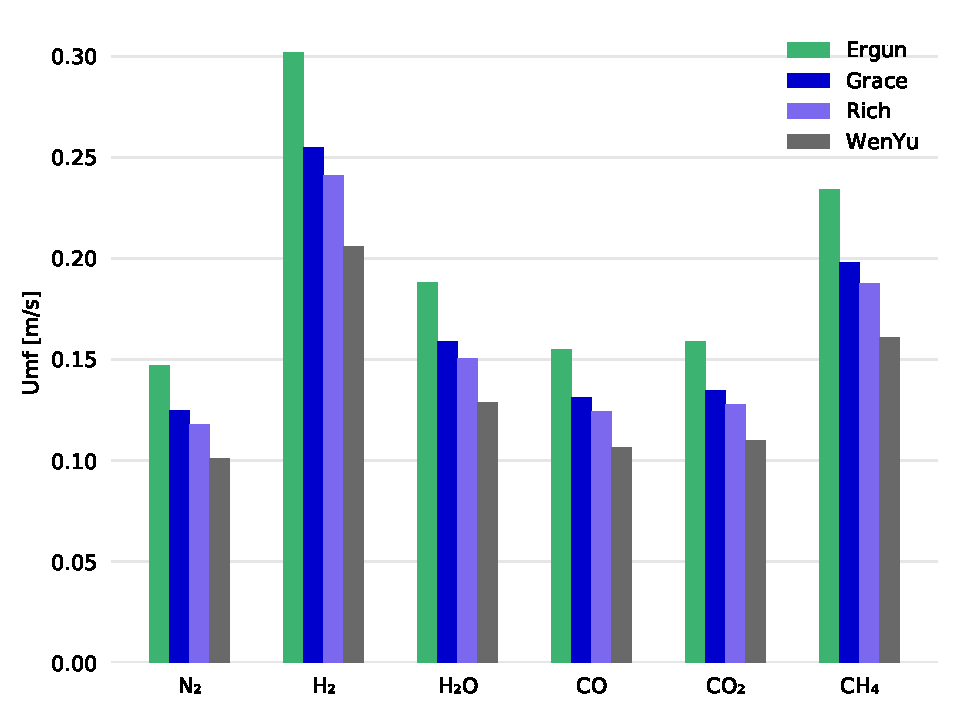
\includegraphics[width=0.8\textwidth]{gas-umf.pdf}
    \caption{Comparison of minimum fluidization velocity (Umf) for different fluidization gases. Values calculated with the Ergun, Grace, Richardson, and Wen and Yu correlations.}
    \label{fig:gas-umf}
\end{figure}

\subsection{Evaluation of the kinetic scheme}

The Di Blasi kinetics were put to use in a batch reactor model to investigate the time scales associated with the reaction mechanisms. Figure \ref{fig:batch-blasi} is an overview of the biomass conversion and product yields using the Di Blasi kinetics in a batch reactor at 773.15 K (500$^\circ$C). At this temperature, without the effects of secondary reactions, the kinetics offer a maximum achievable tar yield of 78\% within 5 seconds. However, if secondary reactions occur during the entire pyrolysis process then a maximum tar yield of only 53\% is possible. The Di Blasi kinetics suggest that minimizing the extent of secondary reactions is critical to producing the maximum possible tar yield.

A range of reaction temperatures were applied to the Di Blasi kinetics in the batch reactor model as shown in Figure \ref{fig:batch-blasi-temps}. The kinetics suggest that temperature has a neglible effect on primary tar yield but effects of secondary reactions are more pronounced. When secondary reactions occur during the entire pyrolysis process, maximum tar yields are realized at higher temperatures but with shorter residence times. These results suggest that if secondary reactions are minimized then temperature should not have a drastic effect on tar yield.

\begin{figure}[H]
    \centering
    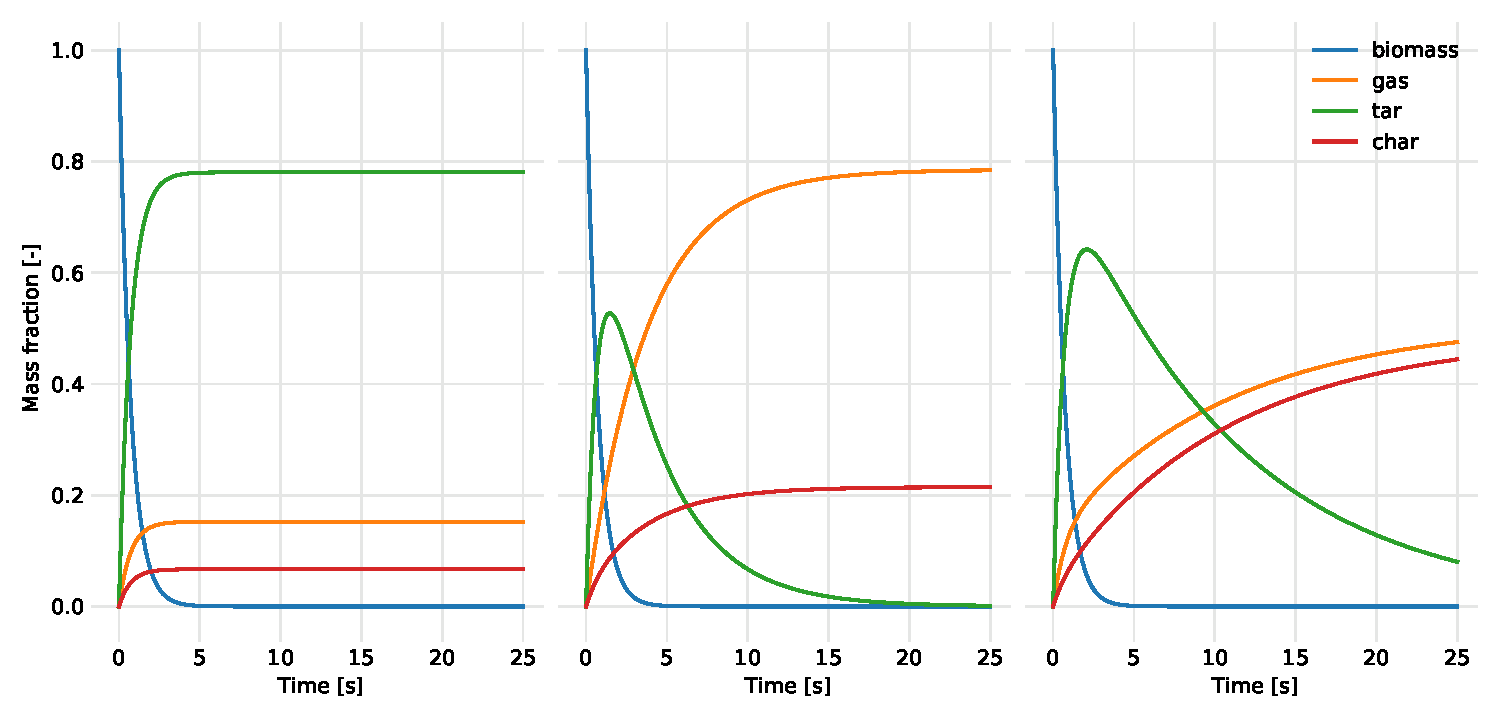
\includegraphics[width=\textwidth]{batch-blasi.pdf}
    \caption{Biomass conversion and product yields in a batch reactor model at 773.15 K (500$^\circ$C) according to the Di Blasi kinetic reactions. Results shown for primary reactions only (left) along with primary and secondary reactions (right).}
    \label{fig:batch-blasi}
\end{figure}

\begin{figure}[H]
    \centering
    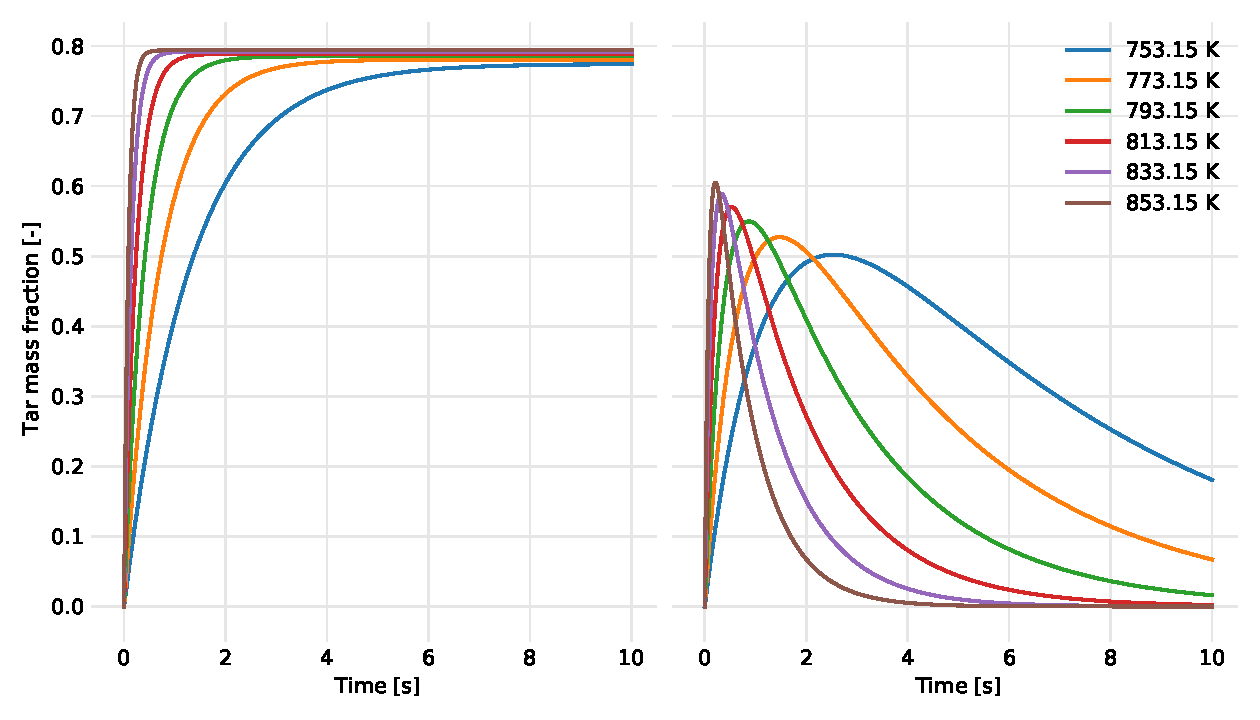
\includegraphics[width=\textwidth]{batch-blasi-temps.pdf}
    \caption{Tar yields for reaction temperatures of 753.15--853.15 K (480--580$^\circ$C) using the Di Blasi kinetics in a batch reactor model. Results shown for primary tar (left) along with primary and secondary tar (right).}
    \label{fig:batch-blasi-temps}
\end{figure}

\subsection{Comparison of pyrolysis yields}

Here.
